%----------------------------------------------------------------------------
\chapter{Tervezés}
\label{chp:design}
%----------------------------------------------------------------------------
\begin{itemize}
  \item a megoldás működését magyarázó vezérabra bemutatása
  \item metamodell készítésének lépései
\end{itemize}

modell, azon végzett terítési műveletek
- archi - ki kivel kommunikálha, szereplők
- modell szétvágva 3 részre : LABOROK, TÁRGYak, milyen gépre milyen vm-et lehet telepítne, terítési műveletek

a fejezetbe szerepelni fogó ábrák és azoknak a nagyonrövid leírása:



\Aref{fig:designoverview}-es ábra fogja elmagyarázni az új terítési megoldás alapvető működési elvét: beolvassuk a modellt, ami alapján az egyik gépet seed-nek kiválasztva megcsináljuk a torrentes terítés. Az alkalmazás a terítésben szereplő gépektől (a torrent swarm-ja) futás közben a terítés állapotáról kér le információkat.

\begin{figure}[ht]
	\centering
	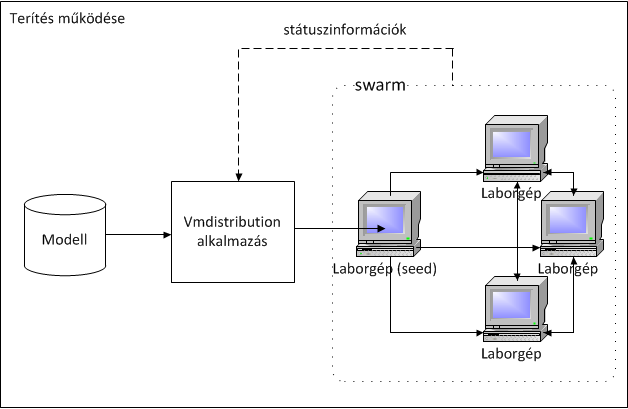
\includegraphics[width=130mm, keepaspectratio]{figures/design_overview.png}
	\caption{}
	\label{fig:designoverview}
\end{figure}

\Aref{fig:designprotocols}-es ábrán látjuk, hogy a terítés egyes szereplői hogyan és milyen protokollokat használva kommunikálnak egymással. [kell-e vajon ehhez, ill. az előzőhöz a tárhely, ahol a virtuális gépeket tároljuk?]

\begin{figure}[ht]
	\centering
	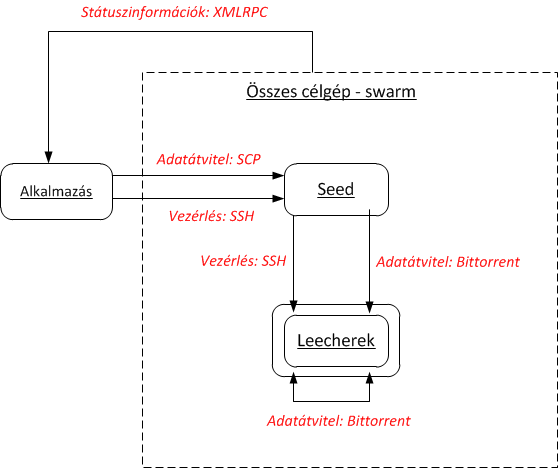
\includegraphics[width=140mm, keepaspectratio]{figures/design_protocols.png}
	\caption{.}
	\label{fig:designprotocols}
\end{figure}

\Aref{fig:designmodelparts}-es ábra mutatja meg, hogy milyen 3 részere vághatjuk a terítéshez szükséges modellt.

\begin{figure}[ht]
	\centering
	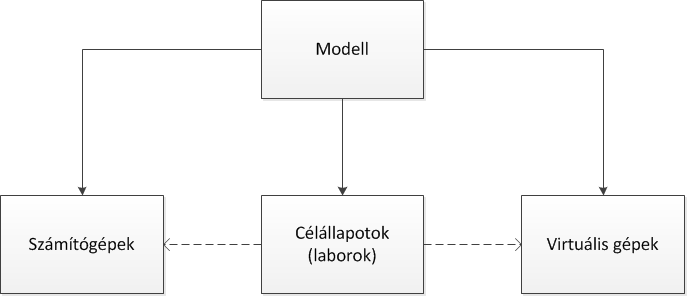
\includegraphics[width=100mm, keepaspectratio]{figures/design_modelparts.png}
	\caption{}
	\label{fig:designmodelparts}
\end{figure}

\Aref{fig:designcomputers}-s ábrán a számítógépeket tartalmazó darab részletesebb leírása van.

\begin{figure}[ht]
	\centering
	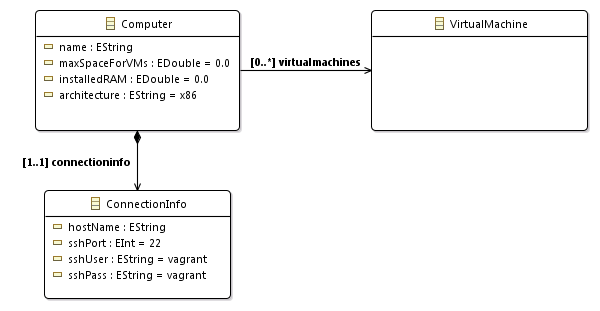
\includegraphics[width=110mm, keepaspectratio]{figures/design_computer.png}
	\caption{}
	\label{fig:designcomputers}
\end{figure}

\Aref{fig:designvm}-s ábrán a virtuális gépeket tartalmazó darab részletesebb leírása van.

\begin{figure}[ht]
	\centering
	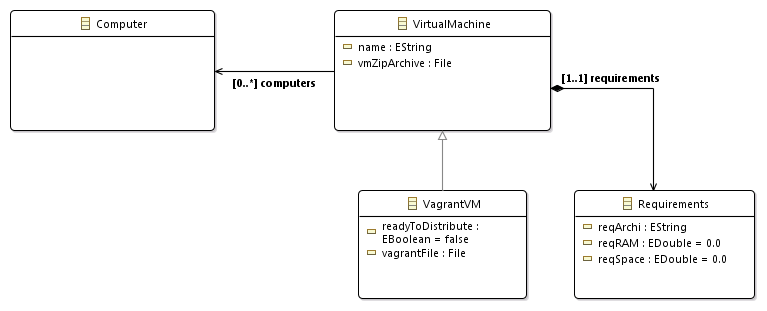
\includegraphics[width=130mm, keepaspectratio]{figures/design_vm.png}
	\caption{}
	\label{fig:designvm}
\end{figure}

\Aref{fig:designlab}-s ábrán a terítés végállapotát (pc->vm összerendelések) tartalmazó darab részletesebb leírása van.

\begin{figure}[ht]
	\centering
	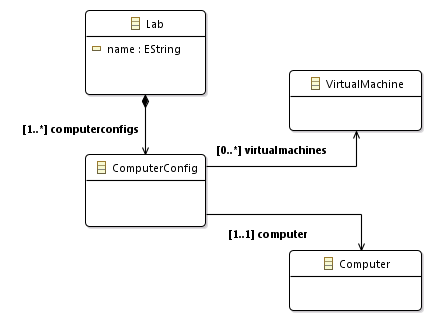
\includegraphics[width=100mm, keepaspectratio]{figures/design_lab.png}
	\caption{}
	\label{fig:designlab}
\end{figure}

% %----------------------------------------------------------------------------
% \section{Követelmények}
% %----------------------------------------------------------------------------
% \begin{itemize}
%   \item feladatkiírás alapján mik a követelmények, az alkalmazásnak milyen funkciókat kell megvalósítania
% \end{itemize}
% 
% %----------------------------------------------------------------------------
% \section{Metamodell}
% %----------------------------------------------------------------------------
% 
% \begin{itemize}
%   \item modell tervezése és készítése, hogyan épül fel/milyen szempontok alapján készült\ldots
% \end{itemize}
% 
% %----------------------------------------------------------------------------
% \section{Az alkalmazás architektúrája}
% %----------------------------------------------------------------------------
% 
% %
% \subsection{Tervezési döntések}
% %
% \begin{itemize}
%   \item fontosabb tervezési döntések leírása( pl.miért nincs grafikus felhasználói felület)
% \end{itemize}
% 
% %
% \subsection{Az alkalmazás komponensei}
% %
% \begin{itemize}
%   \item egyes komponensek bemutatása (uml diagramok ide)
% \end{itemize}